\documentclass[pdf]{beamer}

\usepackage{amsmath}
\usepackage{amsfonts}

\usepackage{graphics,graphicx,subfigure,color}

\usepackage{tikz} % graphical models
\usetikzlibrary{chains,fit,shapes}
\usetikzlibrary{bayesnet}


\mode<presentation>{}

\title{Extended Topic Models with Numerical Features}

\author{G\" okhan \c Capan, Ali Caner T\" urkmen}
\begin{document}
	
\begin{frame}
	\titlepage
\end{frame}

\begin{frame}{Introduction: Topic Models}
	
	\begin{itemize}
		\item {\em Unsupervised} learning, recover \emph{latent} topics in documents
		\item Can be thought of as {\em clustering}.
		\item {\bf Key Assumption:} Topics lead to distinct word distributions. Intuitive. 
	\end{itemize}
\end{frame}

\begin{frame}{Latent Dirichlet Allocation}	
	\begin{itemize}
		\item Rich, probabilistic mixed membership model due to \cite{blei_latent_2003}
		\item Widely adopted and extended
		\item Assumes a fixed number of topics in a corpus
		\item {\bf Key Idea: } A document includes words from multiple topics (in contrast with clustering)
	\end{itemize}
\end{frame}

\begin{frame}{LDA - Generative Model}	
	\begin{itemize}
		\item For each document;
		\begin{itemize}
			\item Topic proportions vector is drawn ($\theta \sim Dirichlet(\alpha)$)
			\item For each word in the document
			\begin{itemize}
				\item A topic is drawn from topic proportions ($z_i \sim Multinomial(\theta)$)
				\item The word is drawn from topic ($w_i \sim Multinomial(\beta_{z_i})$)
			\end{itemize}
		\end{itemize}
	\end{itemize}
\end{frame}


\begin{frame}{LDA - Bayesian Network Representation}
	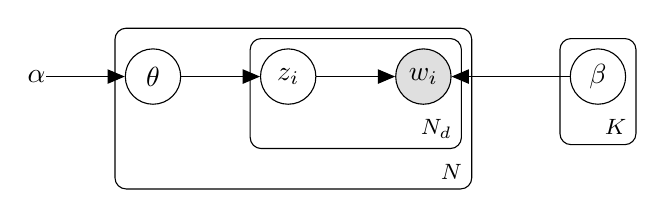
\begin{tikzpicture}
	  \node[latent] (z) {$z_i$} ; %
	  \node[obs, right = of z] (w) {$w_i$};
          \node[latent, left=of z] (theta) {$\theta$} ; %
          \node[const, left=of theta](alpha){$\alpha$};
          \node[latent, right=1.5 of w] (beta) {$\beta$};
        
          \edge {theta} {z} ; %
          \edge {z} {w} ;
          \edge {beta}{w} ;
          \edge {alpha}{theta}
          
          \plate {words}{
          	(z)
		(w)
	  }{$N_d$}
	  
          \plate {docs} {
          	(theta)
		(words)
          }{$N$}
          
          \plate {topicwords}{
          	(beta)
	 }{$K$}
    
	\end{tikzpicture}
	\hspace{5cm}
	\begin{itemize}
		\item Note the difference with document clustering ($z$ is outside of the plate in that case, each word of a document comes from a single cluster), which is referred to as \textit{mixture of unigrams}
	\end{itemize}
\end{frame}

\begin{frame}{LDA - Multi Modal (Aspect) Variants}
	\begin{itemize}
		\item A topic generates not only words, but also other modalities
		\item The features can be paired with words themselves (e.g. sentiment, polarity, word sense disambiguation)
		\item The topics can generate other aspects
		\item Some examples:
		\begin{itemize}
			\item \cite{putthividhy_topic_2010} in CVPR.
			\item \cite{roller_multimodal_2013} in ACL/EMNLP.
			\item \cite{troelsga_ard_topic_2014} in NIPS workshop. 
		\end{itemize}
	\end{itemize}
\end{frame}

\begin{frame}{Multi-Modal LDA Variants}
	\begin{figure}
	\begin{tabular}{cccc}
	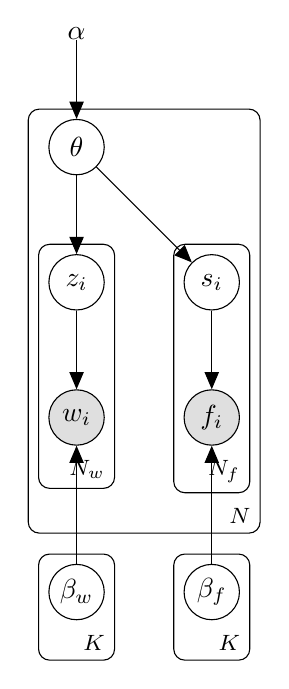
\begin{tikzpicture}
	  \node[latent] (z) {$z_i$} ; %
	  \node[latent, right = of z](z2) {$s_i$};
	  
	  \node[obs, below = of z] (w) {$w_i$};
	  \node[obs, below = of z2](w2) {$f_i$};
	  
          \node[latent, above=of z] (theta) {$\theta$} ; %
          \node[const, above=of theta](alpha){$\alpha$};
          \node[latent, below=1.5 of w] (beta) {$\beta_w$};
          \node[latent, below=1.5 of w2](beta2){$\beta_f$};
        
          \edge {theta} {z} ; %
          \edge {theta}{z2} ;
          \edge {z} {w} ;
          \edge{z2}{w2} ;
          \edge {beta}{w} ;
          \edge {alpha}{theta} ;
           \edge {beta2}{w2} ;
          
          \plate {words}{
          	(z)
		(w)
	  }{$N_w$}
	  
	  \plate {wordsm}{
          	(z2)
		(w2)
	  }{$N_f$}

          \plate {docs} {
          	(theta)
		(words)
		(wordsm)
          }{$N$}
          
          \plate {topicwords}{
          	(beta)
	 }{$K$}
	 
	 \plate {topicwords2}{
          	(beta2)
	 }{$K$}

	\end{tikzpicture}
	
	& & &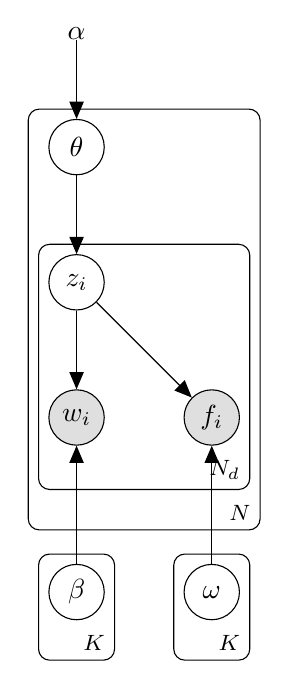
\begin{tikzpicture}
	  \node[latent] (z) {$z_i$} ; %
	  \node[obs, below = of z] (w) {$w_i$};
	  \node[obs, right = of w] (f) {$f_i$};
          \node[latent, above=of z] (theta) {$\theta$} ; %
          \node[const, above=of theta](alpha){$\alpha$};
          \node[latent, below=1.5 of w] (beta) {$\beta$};
          \node[latent, below=1.5 of f] (omega) {$\omega$};
        
          \edge {theta} {z} ; %
          \edge {z} {w} ;
          \edge {z} {f};
          \edge {beta}{w} ;
          \edge {omega}{f}
          \edge {alpha}{theta};
          
          \plate {words}{
          	(z)
		(w)
		(f)
	  }{$N_d$}
	  
          \plate {docs} {
          	(theta)
		(words)
          }{$N$}
          
          \plate {topicwords}{
          	(beta)
	 }{$K$}
	\plate{topicfeatures}{
	 	(omega)
	}{$K$}
	\end{tikzpicture}
	\end{tabular}
	\end{figure}

\end{frame}

\begin{frame}{Proposed Model (Tentative)}
	\begin{tikzpicture}
	  \node[latent] (z) {$z_i$} ; %
	  \node[latent, below=of z](z2) {$s_i$};
	  
	  \node[obs, right=of z] (w) {$w_i$};
	  \node[obs, right=of z2](w2){$C$};
	  
          \node[latent, left=of z] (theta) {$\theta$} ; %
          \node[const, left=of theta](alpha){$\alpha$};
          \node[latent, right=1.5 of w] (beta) {$\beta$};
          \node[latent, below=of beta](lambda){$\lambda$};
        
          \edge {theta} {z} ; %
          \edge {theta}{z2} ;
          \edge {z2}{w2} ;
          \edge {z} {w} ;
          \edge {beta}{w} ;
          \edge {alpha}{theta} ;
           \edge {lambda}{w2} ;
          
          \plate {words}{
          	(z)
		(w)
	  }{$N_w$}
	  
	  \plate {features}{
	  	(z2)
	  	(w2)
	  }{$N_f$}
	  
          \plate {docs} {
          	(theta)
		(words)
		(wordsm)
          }{$N$}
          
          \plate {topicwords}{
          	(beta)
	 }{$K$}
	 
	 \plate {topicwords2}{
          	(lambda)
	 }{$K$}
	 
	\end{tikzpicture}
	\begin{itemize}
		  \item Here, $C$ is an $|L|$ dimensional vector of Poisson random variables, where $L$ is the set of numerical features
	\end{itemize}
\end{frame}



\begin{frame}{Data Set and Features}
	
	\begin{itemize}
		\item {\bf Data Set:} News articles sampled from Anadolu Agency website. 1337 documents (can be expanded), ~3000 tokens after adjusting for document frequency. 
		\item {\bf Features:} Complexity features such as word count, sentence count, average sentence length, comma count. (TBD)
		\item {\bf Novel Features:} Etymological counts. Count the number of words from their etymological origins. Number of Arabic, Farsi, French words, etc. Source: TR Wiktionary Database Dump.
	\end{itemize}
	
\end{frame}

\begin{frame}{Learning}
	
	\begin{itemize}
		\item {\bf Variational inference: } Derive approximate inference algorithms based on a decoupling of the original model OR Variational EM-like procedures to find parameter estimates.
		\item Gibbs sampling assuming appropriate priors (tentative, out of scope for this project)
	\end{itemize}
	
\end{frame}

\begin{frame}{Conclusion}
	
	We propose two key contributions
	\begin{itemize}
		\item Put the topic modeling problem in an extended LDA framework, with numerical features
		\item Use etymological counts for the Turkish language
	\end{itemize}
	
\end{frame}

\begin{frame}{}
	
	Thank You!
	
	\hspace{5cm}
	
	gokhan.capan [at] boun.edu.tr
	
	caner.turkmen [at] boun.edu.tr
	
\end{frame}

\bibliography{caner}{}
\bibliographystyle{apalike}



\begin{frame}{Coupled Matrix Factorization for Recovering Topics}
	
	\begin{figure}[h]
		\centering
		\includegraphics[width=9cm]{images/nmf2.png}
	\end{figure}
	
	\begin{itemize}
		
		\item Represent data with well-known algebraic structures
		\item Jointly guide topic assignments from multimodal datasets, in a probabilistically sound framework
		\item Easily extensible to semi-supervised learning, kernel methods
		\item (T. and Cemgil, 2016)
	\end{itemize}
	
\end{frame}

\begin{frame}{Extended Coupled NMF for Topic Learning with Count Features}
	
	\begin{figure}[h]
		\centering
		\includegraphics[width=7cm]{images/ext_nmf.png}
	\end{figure}
	
	\begin{itemize}
		\item $ y_{ij} | W, H \sim GPO(\sum_{t} w_{it} h_{tj}, \phi) $
		\item $ x_{kj} | V, H \sim GPO(\sum_{t} v_{kt} h_{tj}, \gamma) $
		\item Guide topic modeling with numeric count data
		\item Can assume priors $p(W), p(H), p(V)$ for Bayesian learning
	\end{itemize}
	
\end{frame}

\end{document}